\chapter{Pr\'eliminaires -- Notions de base en \'electronique}

\section{Savoir lire un sch\'ema \'electronique}\label{sec:schematic}

Lire un sch\'ema \'electronique consiste à interpr\'eter un ensemble de symboles normalis\'es
qui repr\'esentent les composants, ainsi que leurs connexions entre eux.
Un sch\'ema ne montre pas l’agencement physique des composants sur une carte, mais leur
relation \'electrique. Comme le plan du m\'etro, les distances et angles ne sont pas
à l’\'echelle, mais les connexions sont correctes.

\subsection{Les symboles de base}

Chaque composant est repr\'esent\'e par un symbole normalis\'e, les symboles seront pr\'esent\'es
au fur et à mesure dans le document.
Voici quelques exemples de symboles courants :
\begin{itemize}
    \item \textbf{R\'esistance} :
    \raisebox{-0.5\height}{%
        \begin{circuitikz}
            \draw (0,0) to[R] (2,0);
        \end{circuitikz}
    }

    \item \textbf{Condensateur} :
    \raisebox{-0.5\height}{%
        \begin{circuitikz}
            \draw (0,0) to[C] (2,0);
        \end{circuitikz}
    }

    \item \textbf{Diode} :
    \raisebox{-0.5\height}{%
        \begin{circuitikz}
            \draw (0,0) to[D] (2,0);
        \end{circuitikz}
    }

    \item \textbf{Transistor NPN} :
    \raisebox{-0.5\height}{%
        \begin{circuitikz}
            \draw (0,0) to[short, o-o] (2,0);
            \draw (1,0) node[npn, anchor=B, rotate=0]{};
        \end{circuitikz}
    }

    \item \textbf{Source de tension} :
    \raisebox{-0.5\height}{%
        \begin{circuitikz}
            \draw (0,0) to[V] (2,0);
        \end{circuitikz}
    }

    \item \textbf{Source de courant} :
    \raisebox{-0.5\height}{%
        \begin{circuitikz}
            \draw (0,0) to[I] (2,0);
        \end{circuitikz}
    }

    \item \textbf{Masse} :
    \raisebox{-0.5\height}{%
        \begin{circuitikz}
            \draw (0,0) node[ground]{};
        \end{circuitikz}
    }

    \item \textbf{Op-amp} :
    \raisebox{-0.5\height}{%
        \begin{circuitikz}
            \draw (0,0) node[op amp, anchor=-] {};
        \end{circuitikz}
    }

    \item \textbf{Inductance} :
    \raisebox{-0.5\height}{%
        \begin{circuitikz}
            \draw (0,0) to[L] (2,0);
        \end{circuitikz}
    }

    \item \textbf{Interrupteur} :
    \raisebox{-0.5\height}{%
        \begin{circuitikz}
            \draw (0,0) to[spst] (2,0);
        \end{circuitikz}
    }
\end{itemize}

\subsection{Les connexions et nœuds}

Les fils reliant les symboles indiquent les conducteurs \'electriques.
Un point marqu\'e par un \textbf{nœud} (un petit rond noir) repr\'esente une connexion entre plusieurs fils.
En revanche, deux fils qui se croisent sans point ne sont pas connect\'es.

\begin{figure}[H]
  \centering
  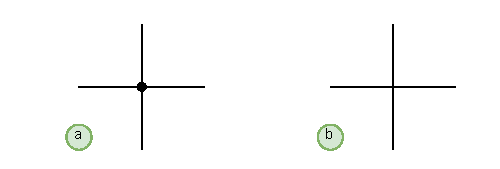
\includegraphics[width=0.8\textwidth]{wires.pdf}
  \caption{\fakecustommacro{a} : fils connect\'es avec un nœud. \fakecustommacro{b} : fils crois\'es sans connexion.}
\end{figure}


\subsection{Fl\'echage des tensions et des courants}
Pour analyser un circuit, il est souvent utile de fl\'echer les tensions et les courants.
\begin{itemize}
    \item \textbf{Tension} : La tension est une diff\'erence de potentiel entre deux points.
    On flèche la tension de la borne positive (\(+\)) vers la borne n\'egative (\(-\)).
    \item \textbf{Courant} : Le courant est le flux de charges \'electriques.
    On flèche le courant dans la direction du flux des charges positives (de \(+\) vers \(-\)).
\end{itemize}
Ces flèches aident à visualiser comment l’\'energie circule dans le circuit.

\subsection{Exemple simple}

\begin{figure}[H]
    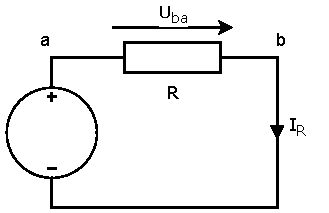
\includegraphics[width=0.7\textwidth]{example-schema.pdf}
    \caption{
        Un sch\'ema de maille simple avec une source de tension et une r\'esistance
    }
\end{figure}

\subsection{La lecture d’un circuit}

\begin{Note}
Pour lire un sch\'ema, on suit g\'en\'eralement ces \'etapes :
\begin{enumerate}
  \item Identifier la source d’\'energie (pile, alimentation).
  \item Rep\'erer la masse (r\'ef\'erence commune du circuit), si elle est pr\'esente.
  \item Suivre le parcours du courant à travers les composants.
  \item Reconna\^itre les sous-circuits classiques : diviseur de tension, filtre RC, pont redresseur, etc.
\end{enumerate}

Pour une analyse d'un circuit complexe, on peut ignorer les valeurs des composants et se concentrer sur la topologie du circuit,
c'est-à-dire rep\'erer comment les montages courants comme les redresseurs, amplificateurs, oscillateurs, etc. sont interconnect\'es.
\end{Note}

\section{Concepts \'electriques de base}
\subsection{Admittance, Imp\'edance, Conductance et Résistance}
\begin{itemize}
    \item \textbf{Résistance (R)} : La résistance est une mesure de l’opposition au flux de courant dans un conducteur.
    Elle est mesurée en ohms (\(\Omega\)) et est définie par la loi d’Ohm : \(V = IR\), où \(V\) est la tension, \(I\) le courant, et \(R\) la résistance.\footnote{Concept d\'evelopp\'e en section \Cref{subsec:resistors}.}
    \item \textbf{Conductance (G)} : La conductance est l’inverse de la résistance, mesurée en siemens (S).
    Elle indique la facilité avec laquelle le courant peut circuler à travers un matériau : \(G = \frac{1}{R}\).
    \item \textbf{Impedance (Z)} : L’impédance est une généralisation de la résistance pour les circuits en courant alternatif (AC).
    Elle combine la résistance et la réactance (due aux condensateurs et inducteurs) et est également mesurée en ohms (\(\Omega\)).
    L’impédance est une quantité complexe, exprimée comme \(Z = R + jX\), où \(X\) est la réactance.
    \item \textbf{Admittance (Y)} : L’admittance est l’inverse de l’impédance, mesurée en siemens (S).
    Elle combine la conductance et la susceptance (l’inverse de la réactance) : \(Y = G + jB\), où \(B\) est la susceptance.
\end{itemize}
